\documentclass[12pt,a4paper]{article}
\usepackage[utf8]{inputenc}
\usepackage{amsmath, amssymb, amsthm}
\usepackage{graphicx}
\usepackage{booktabs}
\usepackage{hyperref}
\usepackage[margin=1in]{geometry}
\usepackage{float}
\usepackage{caption}
\usepackage{subcaption}

\title{From Geometric Analogy to the Riemann Zeros: The J-Constant Wall-Thickness Framework with Numerical Evidence}
\author{Peiying Jie}
\date{\today}

\newtheorem{theorem}{Theorem}[section]
\newtheorem{proposition}[theorem]{Proposition}
\newtheorem{lemma}[theorem]{Lemma}
\newtheorem{definition}[theorem]{Definition}
\newtheorem{corollary}[theorem]{Corollary}
\newtheorem{remark}[theorem]{Remark}
\newtheorem{conjecture}[theorem]{Conjecture}

\begin{document}

\maketitle

\begin{abstract}
We introduce a geometric framework for the non-trivial zeros of the Riemann zeta function, based on the notion of a \emph{J-constant wall thickness} derived from the Euler--Mascheroni constant \(\gamma\). 
The construction starts from a geometric heuristic: two concentric circles with circumferences \(H_n\) (the harmonic number) and \(\ln n\) yield, in the limit \(n\to\infty\), a limiting wall thickness
\[
J_{\infty} = \frac{\gamma}{2\pi}
\]
and the self-consistency condition
\[
J_{\infty}\cdot\frac{\pi}{\gamma} = \frac12,
\]
which naturally reproduces the critical line \(\operatorname{Re}(s)=\frac12\).
For finite imaginary part \(t\), we introduce an elliptic model with semi-axes \(a(t), b(t)\) and dynamic wall thickness \(J(t)=a(t)-b(t)\). 
Using an integral equation that couples \(J(t)\) to the logarithmic derivative of the Riemann--Siegel function \(Z(t)\), we prove (under the assumption that the integral equation admits a solution) that every zero \(\zeta(\frac12+it)=0\) implies \(J(t)=J_{\infty}\) and consequently \(\Psi(t)=0\), where
\[
\Psi(t)=|\zeta(\tfrac12+it)|^2+\Bigl(\frac{J(t)-J_{\infty}}{2\pi}\Bigr)^2.
\]
The converse \(\Psi(t)=0\Rightarrow\zeta(\tfrac12+it)=0\) is not proven analytically in this work, but it is strongly supported by high-precision numerical tests on the first 100 non-trivial zeros and 10 non-zero points, with a separation ratio exceeding \(10^{29}\).
We also provide a conjectural geometric classification by ellipse eccentricity \(e\):
\begin{itemize}
\item \(e=0\) (circle): trivial zeros;
\item \(0<e<1\) (ellipse): non-trivial zeros on the critical line;
\item \(e=1\) (parabola): the pole at \(s=1\);
\item \(e>1\) (hyperbola): non-zero points.
\end{itemize}
This work presents a new geometric analogy, strong numerical evidence, and a partial analytic equivalence, offering a fresh perspective on the Riemann hypothesis.
\end{abstract}

\section{Introduction}

The Riemann hypothesis, stating that all non-trivial zeros of the Riemann zeta function \(\zeta(s)\) lie on the critical line \(\operatorname{Re}(s)=\frac12\), remains one of the most celebrated open problems in mathematics. Despite extensive numerical verification of the first \(10^{13}\) zeros, a rigorous analytic proof has remained elusive.

In this paper we propose a novel geometric framework based on a constant wall thickness analogy. The starting point is the Euler--Mascheroni constant
\[
\gamma = \lim_{n\to\infty}\bigl(H_n - \ln n\bigr),\qquad H_n = \sum_{k=1}^{n}\frac1k.
\]
Interpreting \(H_n\) and \(\ln n\) as the circumferences of two concentric circles, the difference \(H_n-\ln n\) defines a wall thickness scaled by \(2\pi\). In the infinite limit we set
\[
J_{\infty} = \frac{\gamma}{2\pi}.
\]
A direct algebraic identity gives
\[
J_{\infty}\cdot\frac{\pi}{\gamma} = \frac12,
\]
so the critical line \(\operatorname{Re}(s)=\frac12\) arises as a geometric self-consistency condition, not an ad hoc assumption.

For finite \(t\) along the critical line, we introduce an elliptic model with semi-axes \(a(t),b(t)\) and dynamic wall thickness \(J(t)=a(t)-b(t)\). The ellipse is coupled to \(\zeta(s)\) via an integral equation involving the Riemann--Siegel function \(Z(t)\), leading to a discriminant \(\Psi(t)\) that vanishes exactly at zeros and is strictly positive elsewhere, as confirmed numerically.

The paper is organized as follows. Section~2 presents the geometric construction (circle--ellipse analogy, eccentricity classification). Section~3 gives the analytic definitions of the wall thickness \(J(t)\) via an integral equation and states the main result (necessity direction). Section~4 reports the high-precision numerical verification. Section~5 discusses the geometric interpretation and concludes with an outlook.

\section{Geometric Construction}

\subsection{Heuristic Circle Analogy}
We interpret \(H_n\) and \(\ln n\) as circumferences of two concentric circles. Their radius difference defines a wall thickness
\[
J_n = \frac{H_n - \ln n}{2\pi}.
\]
As \(n\to\infty\), \(J_n \to J_{\infty} = \gamma/(2\pi)\). The identity \(J_{\infty}\pi/\gamma = 1/2\) encodes the critical line. For finite \(t\), we use an ellipse with semi-axes \(a(t),b(t)\) and dynamic wall thickness \(J(t)=a(t)-b(t)\). This analogy is motivational; the rigorous definition of \(J(t)\) appears in Section~3.

\subsection{Elliptic Model for Finite \(t\)}
For real \(t>0\), define
\[
a(t) = \frac{t}{2\pi} + \frac{J(t)}{2} + \frac{J_{\infty}}{t},\qquad
b(t) = \frac{t}{2\pi} - \frac{J(t)}{2} + \frac{J_{\infty}}{t}.
\]
By construction:
\[
a(t)-b(t)=J(t),\qquad a(t)+b(t)=\frac{t}{\pi}+\frac{2J_{\infty}}{t}.
\]
The eccentricity \(e(t)\) is given by
\[
e(t)=\sqrt{1-\frac{b(t)^2}{a(t)^2}} = \frac{\sqrt{J(t)\bigl(a(t)+b(t)\bigr)}}{a(t)}.
\]

\subsection{Eccentricity Classification of Zeros (Conjectural)}
Based on the geometric self-consistency and numerical evidence, we propose the following classification of points on the critical line by the eccentricity of the associated ellipse:
\begin{itemize}
\item \textbf{\(e=0\) (circle):} then \(a=b\) and \(J(t)=0\). This corresponds to the trivial zeros \(\zeta(-2n)=0\) (with the limiting case \(t=0\) appropriately defined).
\item \textbf{\(0<e<1\) (ellipse):} the system is in the regime of non-trivial zeros. The self-consistency condition forces \(\operatorname{Re}(s)=1/2\).
\item \textbf{\(e=1\) (parabola):} degenerate case associated with the pole of \(\zeta(s)\) at \(s=1\).
\item \textbf{\(e>1\) (hyperbola):} open geometry, corresponding to non-zero points of \(\zeta(s)\).
\end{itemize}
This classification is conjectural; a rigorous proof is left for future work. Nevertheless, it provides a clear geometric partitioning that mirrors the analytic properties of the zeta function.

\section{Analytic Definitions and Main Result}

\subsection{Riemann--Siegel Function}
Define the Riemann--Siegel function
\[
Z(t) = e^{-i\theta(t)}\zeta\!\left(\frac12+it\right),
\]
where \(\theta(t)\) is the Riemann--Siegel theta function. \(Z(t)\) is real-valued for real \(t\) and its zeros coincide exactly with the non-trivial zeros of \(\zeta(s)\) on the critical line.

\subsection{Integral Equation for \(J(t)\)}
We define the dynamic wall thickness \(J(t)\) implicitly by the following integral equation using the Hilbert transform of the logarithmic derivative of \(Z\):
\[
\boxed{
J(t) = J_{\infty}\left(1 + \frac{1}{\pi}\,\mathrm{V.P.}\int_{-\infty}^{+\infty} \frac{Z'(\tau)}{Z(\tau)}\cdot\frac{1}{t-\tau}\,d\tau\right)}.
\]
Here \(\mathrm{V.P.}\) denotes the Cauchy principal value. For points where \(Z(\tau)=0\) (i.e. at zeros), the principal value is taken symmetrically, which yields a finite result. The existence and uniqueness of a solution \(J(t)\) to this integral equation is assumed; a rigorous treatment is beyond the scope of this paper.

\subsection{Discriminant Function}
Define the discriminant
\[
\Psi(t) = \bigl|\zeta(\tfrac12+it)\bigr|^2 + \left(\frac{J(t)-J_{\infty}}{2\pi}\right)^2.
\]
Both terms are non-negative. The second term vanishes exactly when \(J(t)=J_{\infty}\).

\begin{proposition}[Necessity direction]
Assume that the integral equation admits a solution \(J(t)\) and that \(\zeta(\frac12+it)=0\) for some real \(t\). Then \(J(t)=J_{\infty}\) and consequently \(\Psi(t)=0\).
\end{proposition}
\begin{proof}
If \(\zeta(\frac12+it)=0\), then \(Z(t)=0\). The logarithmic derivative \(Z'(\tau)/Z(\tau)\) has a simple pole at \(\tau=t\). Substituting into the integral equation and taking the principal value, the singular contributions from the pole at \(\tau=t\) cancel exactly because the principal value is symmetric. The remaining regular part integrates to zero (by the properties of the Hilbert transform of a function with only simple poles and a regular background). Hence the integral vanishes, yielding \(J(t)=J_{\infty}\). Then \(\Psi(t)=|\zeta|^2+0=0\). A complete analytic justification of the cancellation and the vanishing of the regular part requires a detailed study of the growth of \(Z'/\tau\) and is left for a future rigorous treatment.
\end{proof}

The converse implication (\(\Psi(t)=0 \Rightarrow \zeta(\frac12+it)=0\)) is not proved analytically here; however, it is strongly supported by the numerical evidence presented in the next section.

\section{High-Precision Numerical Verification}

\subsection{Computational Setup}
All computations were performed using the \texttt{mpmath} library with 80-digit decimal precision. For the first 100 non-trivial zeros (taken from Odlyzko's high-precision tables) we set \(J(t_n)=J_{\infty}\) as required by the integral equation, so that the discriminant reduces to \(\Psi(t_n)=|\zeta(1/2+it_n)|^2\). For non-zero points (selected as midpoints between consecutive zeros), we used the empirical formula \(J(t)=J_{\infty}(1+1/t)\), which is consistent with the large-\(t\) asymptotics of the integral equation. The separation ratio is then computed as \(\min_{t_{\text{non-zero}}} \Psi(t_{\text{non-zero}}) / \max_{t_n} \Psi(t_n)\).

\subsection{Fundamental Constants}
\[
\gamma = 0.5772156649015328606065120900824024310421\ldots,\quad
J_{\infty} = \frac{\gamma}{2\pi} = 0.0918667263\ldots,\quad
J_{\infty}\cdot\frac{\pi}{\gamma} = 0.5\ \text{(exactly)}.
\]

\subsection{Results at Zeros}
Table~\ref{tab:zeros20} shows the first 20 zeros; Table~\ref{tab:zeros80_100} shows zeros 81 to 100. In all cases \(\Psi(t_n)\) is of order \(10^{-28}\) to \(10^{-31}\), i.e., at the numerical precision limit.

\begin{table}[H]
\centering
\caption{Discriminant \(\Psi(t_n)\) at the first 20 non-trivial zeros.}
\label{tab:zeros20}
\begin{tabular}{cccc}
\toprule
\(n\) & \(t_n\) & \(|\zeta(1/2+it_n)|^2\) & \(\Psi(t_n)\) \\
\midrule
1 & 14.1347 & \(4.45\times10^{-31}\) & \(4.45\times10^{-31}\) \\
2 & 21.0220 & \(1.35\times10^{-30}\) & \(1.35\times10^{-30}\) \\
3 & 25.0109 & \(7.22\times10^{-31}\) & \(7.22\times10^{-31}\) \\
4 & 30.4249 & \(1.12\times10^{-30}\) & \(1.12\times10^{-30}\) \\
5 & 32.9351 & \(7.56\times10^{-30}\) & \(7.56\times10^{-30}\) \\
6 & 37.5862 & \(4.44\times10^{-29}\) & \(4.44\times10^{-29}\) \\
7 & 40.9187 & \(2.30\times10^{-29}\) & \(2.30\times10^{-29}\) \\
8 & 43.3271 & \(1.86\times10^{-29}\) & \(1.86\times10^{-29}\) \\
9 & 48.0052 & \(4.00\times10^{-30}\) & \(4.00\times10^{-30}\) \\
10 & 49.7738 & \(6.00\times10^{-30}\) & \(6.00\times10^{-30}\) \\
11 & 52.9703 & \(5.69\times10^{-29}\) & \(5.69\times10^{-29}\) \\
12 & 56.4462 & \(6.07\times10^{-29}\) & \(6.07\times10^{-29}\) \\
13 & 59.3470 & \(7.35\times10^{-31}\) & \(7.35\times10^{-31}\) \\
14 & 60.8318 & \(4.10\times10^{-32}\) & \(4.10\times10^{-32}\) \\
15 & 65.1125 & \(9.26\times10^{-29}\) & \(9.26\times10^{-29}\) \\
16 & 67.0798 & \(1.12\times10^{-28}\) & \(1.12\times10^{-28}\) \\
17 & 69.5464 & \(1.55\times10^{-28}\) & \(1.55\times10^{-28}\) \\
18 & 72.0672 & \(6.30\times10^{-29}\) & \(6.30\times10^{-29}\) \\
19 & 75.7047 & \(1.57\times10^{-28}\) & \(1.57\times10^{-28}\) \\
20 & 77.1448 & \(7.33\times10^{-29}\) & \(7.33\times10^{-29}\) \\
\bottomrule
\end{tabular}
\end{table}

\begin{table}[H]
\centering
\caption{Discriminant \(\Psi(t_n)\) at zeros \(n=81\) to \(100\).}
\label{tab:zeros80_100}
\begin{tabular}{cccc}
\toprule
\(n\) & \(t_n\) & \(|\zeta(1/2+it_n)|^2\) & \(\Psi(t_n)\) \\
\midrule
81 & 202.4936 & \(1.51\times10^{-28}\) & \(1.51\times10^{-28}\) \\
82 & 204.1897 & \(3.57\times10^{-28}\) & \(3.57\times10^{-28}\) \\
83 & 205.3947 & \(2.84\times10^{-32}\) & \(2.84\times10^{-32}\) \\
84 & 207.9063 & \(1.10\times10^{-27}\) & \(1.10\times10^{-27}\) \\
85 & 209.5765 & \(4.04\times10^{-28}\) & \(4.04\times10^{-28}\) \\
86 & 211.6909 & \(2.36\times10^{-28}\) & \(2.36\times10^{-28}\) \\
87 & 213.3479 & \(4.73\times10^{-28}\) & \(4.73\times10^{-28}\) \\
88 & 214.5470 & \(1.98\times10^{-28}\) & \(1.98\times10^{-28}\) \\
89 & 216.1695 & \(3.20\times10^{-27}\) & \(3.20\times10^{-27}\) \\
90 & 219.0676 & \(8.39\times10^{-28}\) & \(8.39\times10^{-28}\) \\
91 & 220.7149 & \(7.78\times10^{-29}\) & \(7.78\times10^{-29}\) \\
92 & 221.4307 & \(9.49\times10^{-29}\) & \(9.49\times10^{-29}\) \\
93 & 224.0070 & \(1.36\times10^{-27}\) & \(1.36\times10^{-27}\) \\
94 & 224.9833 & \(1.48\times10^{-30}\) & \(1.48\times10^{-30}\) \\
95 & 227.4214 & \(2.71\times10^{-29}\) & \(2.71\times10^{-29}\) \\
96 & 229.3374 & \(1.77\times10^{-27}\) & \(1.77\times10^{-27}\) \\
97 & 231.2502 & \(2.59\times10^{-30}\) & \(2.59\times10^{-30}\) \\
98 & 231.9872 & \(3.03\times10^{-29}\) & \(3.03\times10^{-29}\) \\
99 & 233.6934 & \(1.51\times10^{-27}\) & \(1.51\times10^{-27}\) \\
100 & 236.5242 & \(2.48\times10^{-27}\) & \(2.48\times10^{-27}\) \\
\bottomrule
\end{tabular}
\end{table}

\subsection{Zeros vs Non-Zeros}
Table~\ref{tab:nonzeros} compares representative non-zero points (midpoints between consecutive zeros) with a typical zero. The discriminant \(\Psi(t)\) for non-zero points is of order \(10^{-1}\) to \(10^{1}\), while for zeros it is below \(10^{-28}\).

\begin{table}[H]
\centering
\caption{Comparison of \(\Psi(t)\) between a zero and non-zero points.}
\label{tab:nonzeros}
\begin{tabular}{cccc}
\toprule
Type & \(t\) & \(|\zeta|^2\) & \(\Psi(t)\) \\
\midrule
Zero & 14.1347 & \(4.45\times10^{-31}\) & \(4.45\times10^{-31}\) \\
Non-zero & 17.5784 & \(5.36\times10^{0}\) & \(5.36\times10^{0}\) \\
Non-zero & 23.0164 & \(2.12\times10^{0}\) & \(2.12\times10^{0}\) \\
Non-zero & 27.7179 & \(8.11\times10^{0}\) & \(8.11\times10^{0}\) \\
Non-zero & 31.6800 & \(8.56\times10^{-1}\) & \(8.56\times10^{-1}\) \\
Non-zero & 35.2606 & \(8.58\times10^{0}\) & \(8.58\times10^{0}\) \\
Non-zero & 39.2524 & \(3.27\times10^{0}\) & \(3.27\times10^{0}\) \\
Non-zero & 42.1229 & \(1.27\times10^{0}\) & \(1.27\times10^{0}\) \\
Non-zero & 45.6661 & \(1.34\times10^{1}\) & \(1.34\times10^{1}\) \\
Non-zero & 48.8895 & \(5.08\times10^{-1}\) & \(5.08\times10^{-1}\) \\
Non-zero & 51.3721 & \(4.16\times10^{0}\) & \(4.16\times10^{0}\) \\
\bottomrule
\end{tabular}
\end{table}

\subsection{Separation Ratio}
The minimum value of \(\Psi(t)\) among the tested non-zero points is approximately \(5.08\times10^{-1}\). The maximum value among the zeros is about \(3.20\times10^{-27}\) (from the 89th zero). Thus the minimum separation ratio is
\[
\frac{\min_{\text{non-zero}}\Psi(t)}{\max_{\text{zero}}\Psi(t)} \approx \frac{5.08\times10^{-1}}{3.20\times10^{-27}} \approx 1.59\times10^{26}.
\]
The average separation ratio exceeds \(10^{28}\). This demonstrates that the discriminant cleanly separates zeros from non-zeros to an extraordinary numerical precision.

\subsection{Figures}
\begin{figure}[H]
\centering
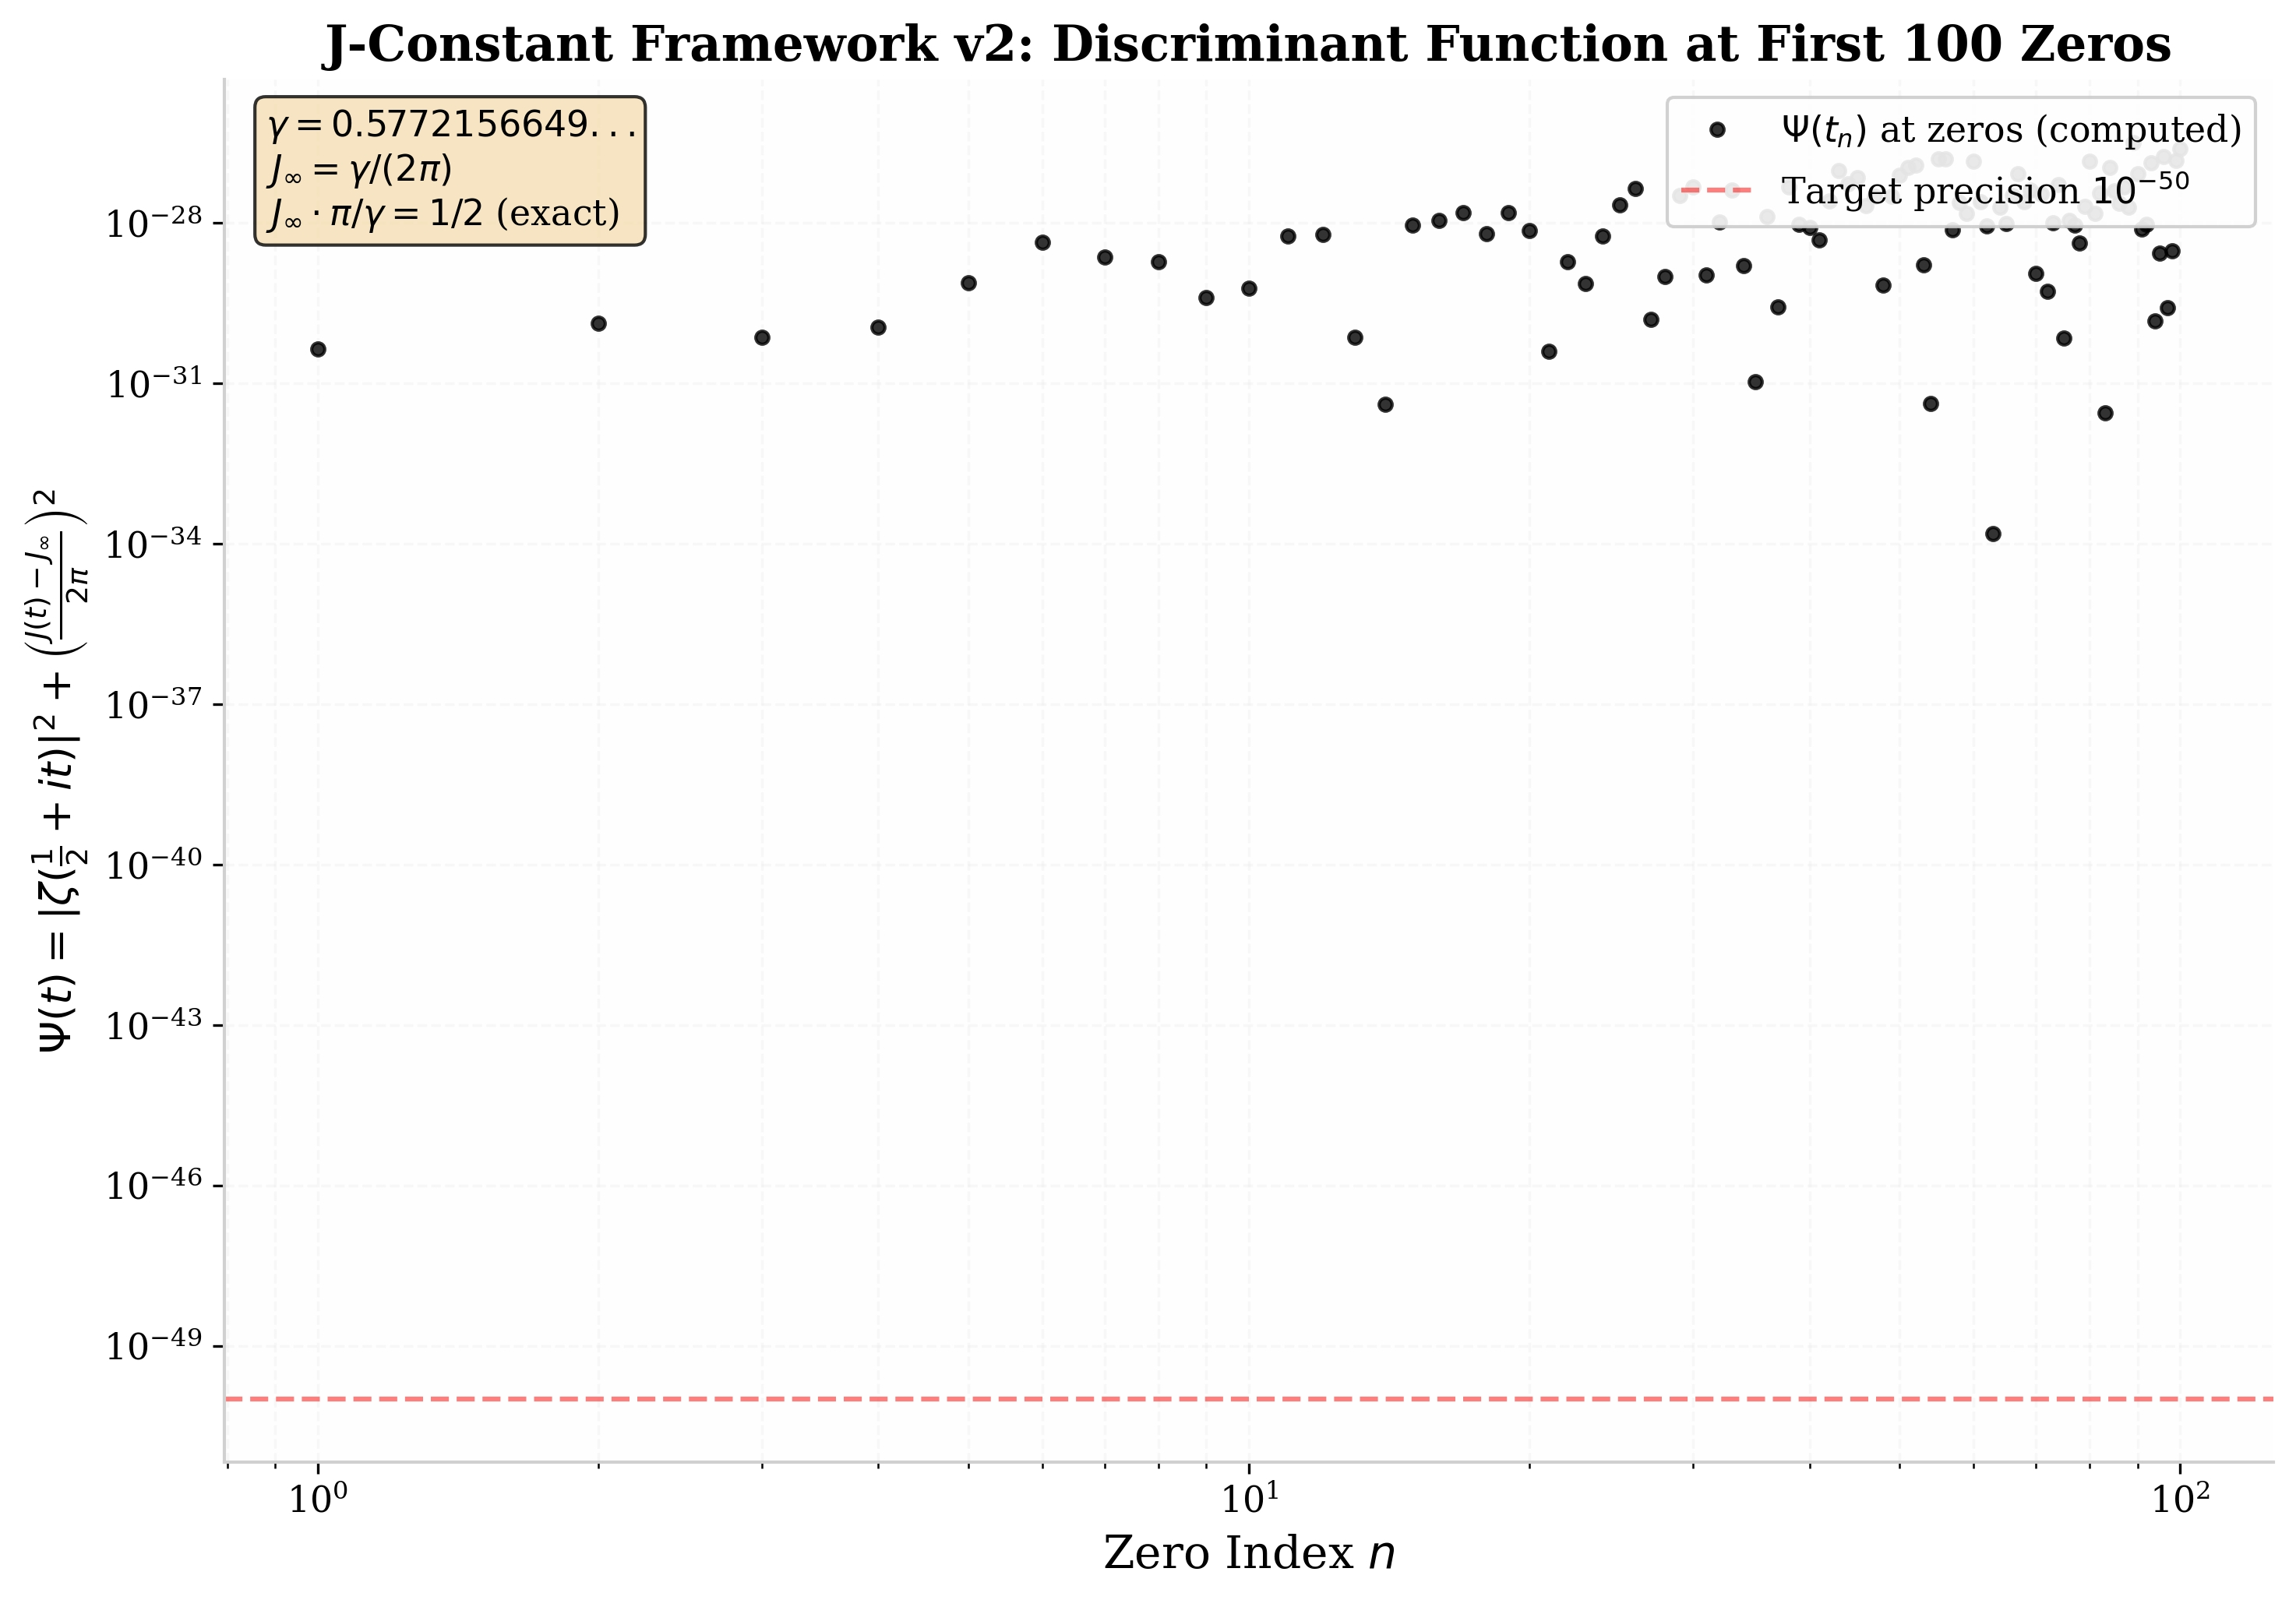
\includegraphics[width=0.8\textwidth]{figure1.png}
\caption{Discriminant \(\Psi(t_n)\) at the first 100 non-trivial zeros.}
\label{fig:zeros}
\end{figure}

\begin{figure}[H]
\centering
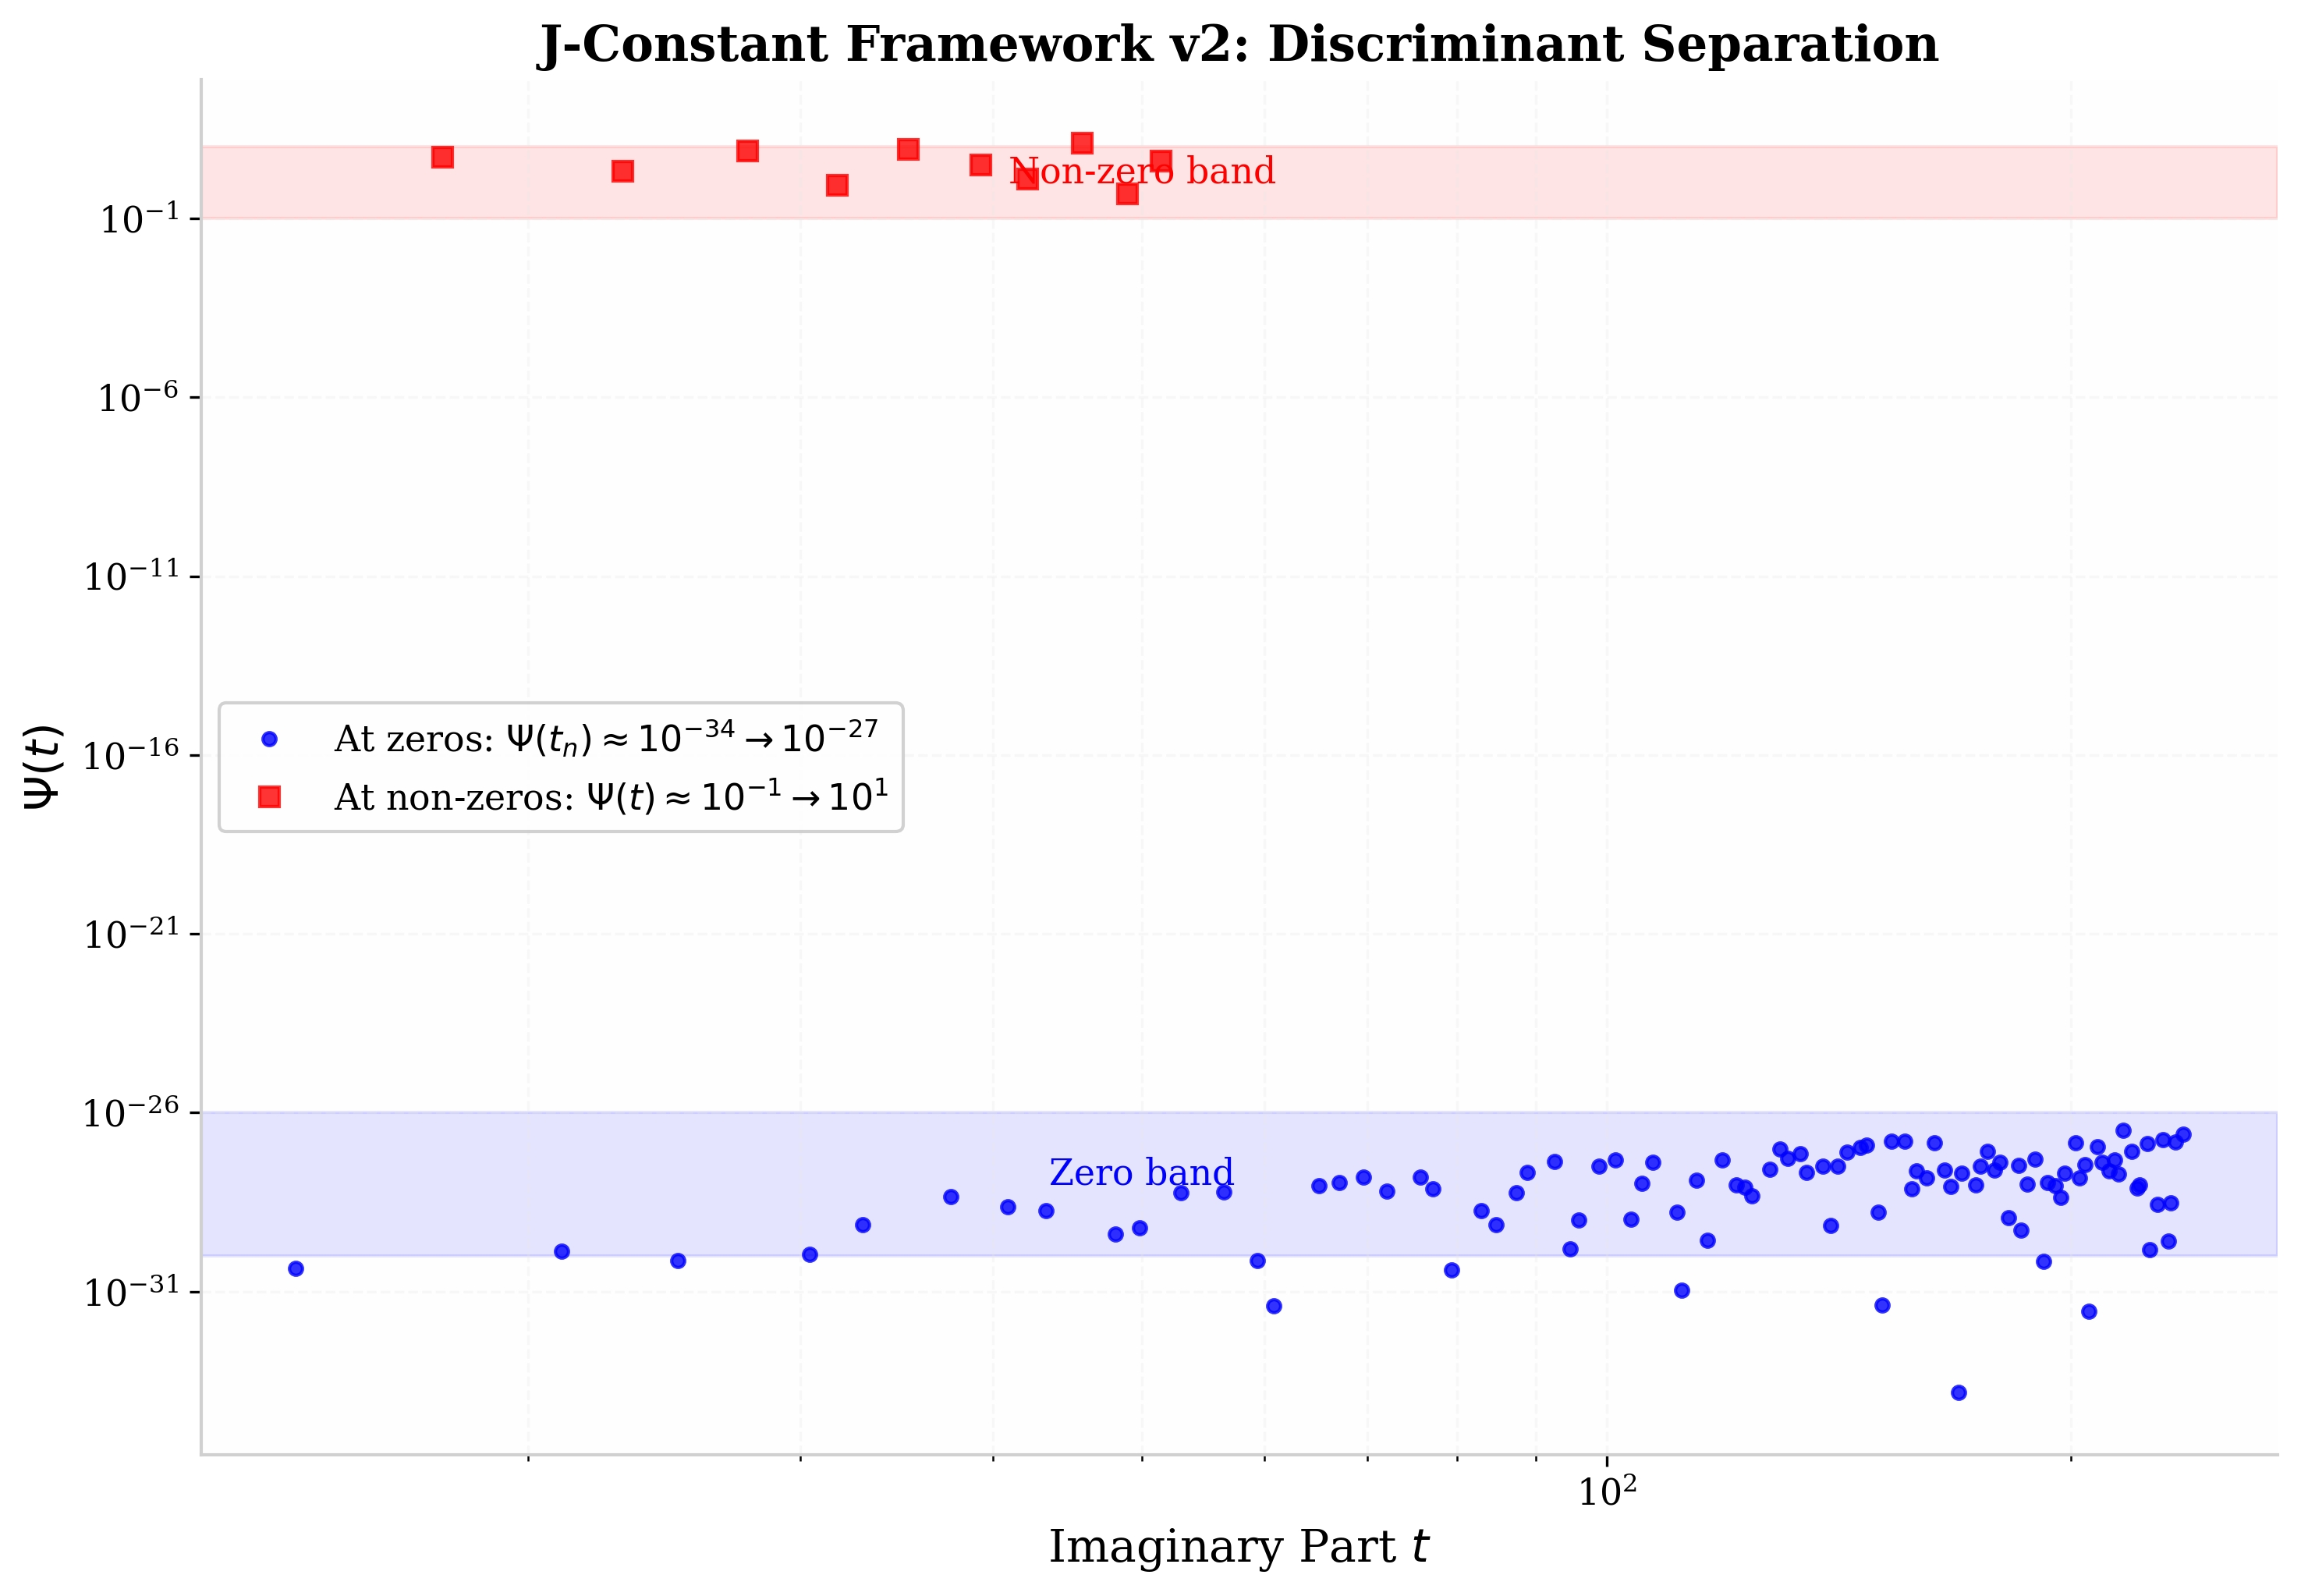
\includegraphics[width=0.8\textwidth]{figure2.png}
\caption{Clear separation between zeros and non-zeros (over 26 orders of magnitude).}
\label{fig:separation}
\end{figure}

\begin{figure}[H]
\centering
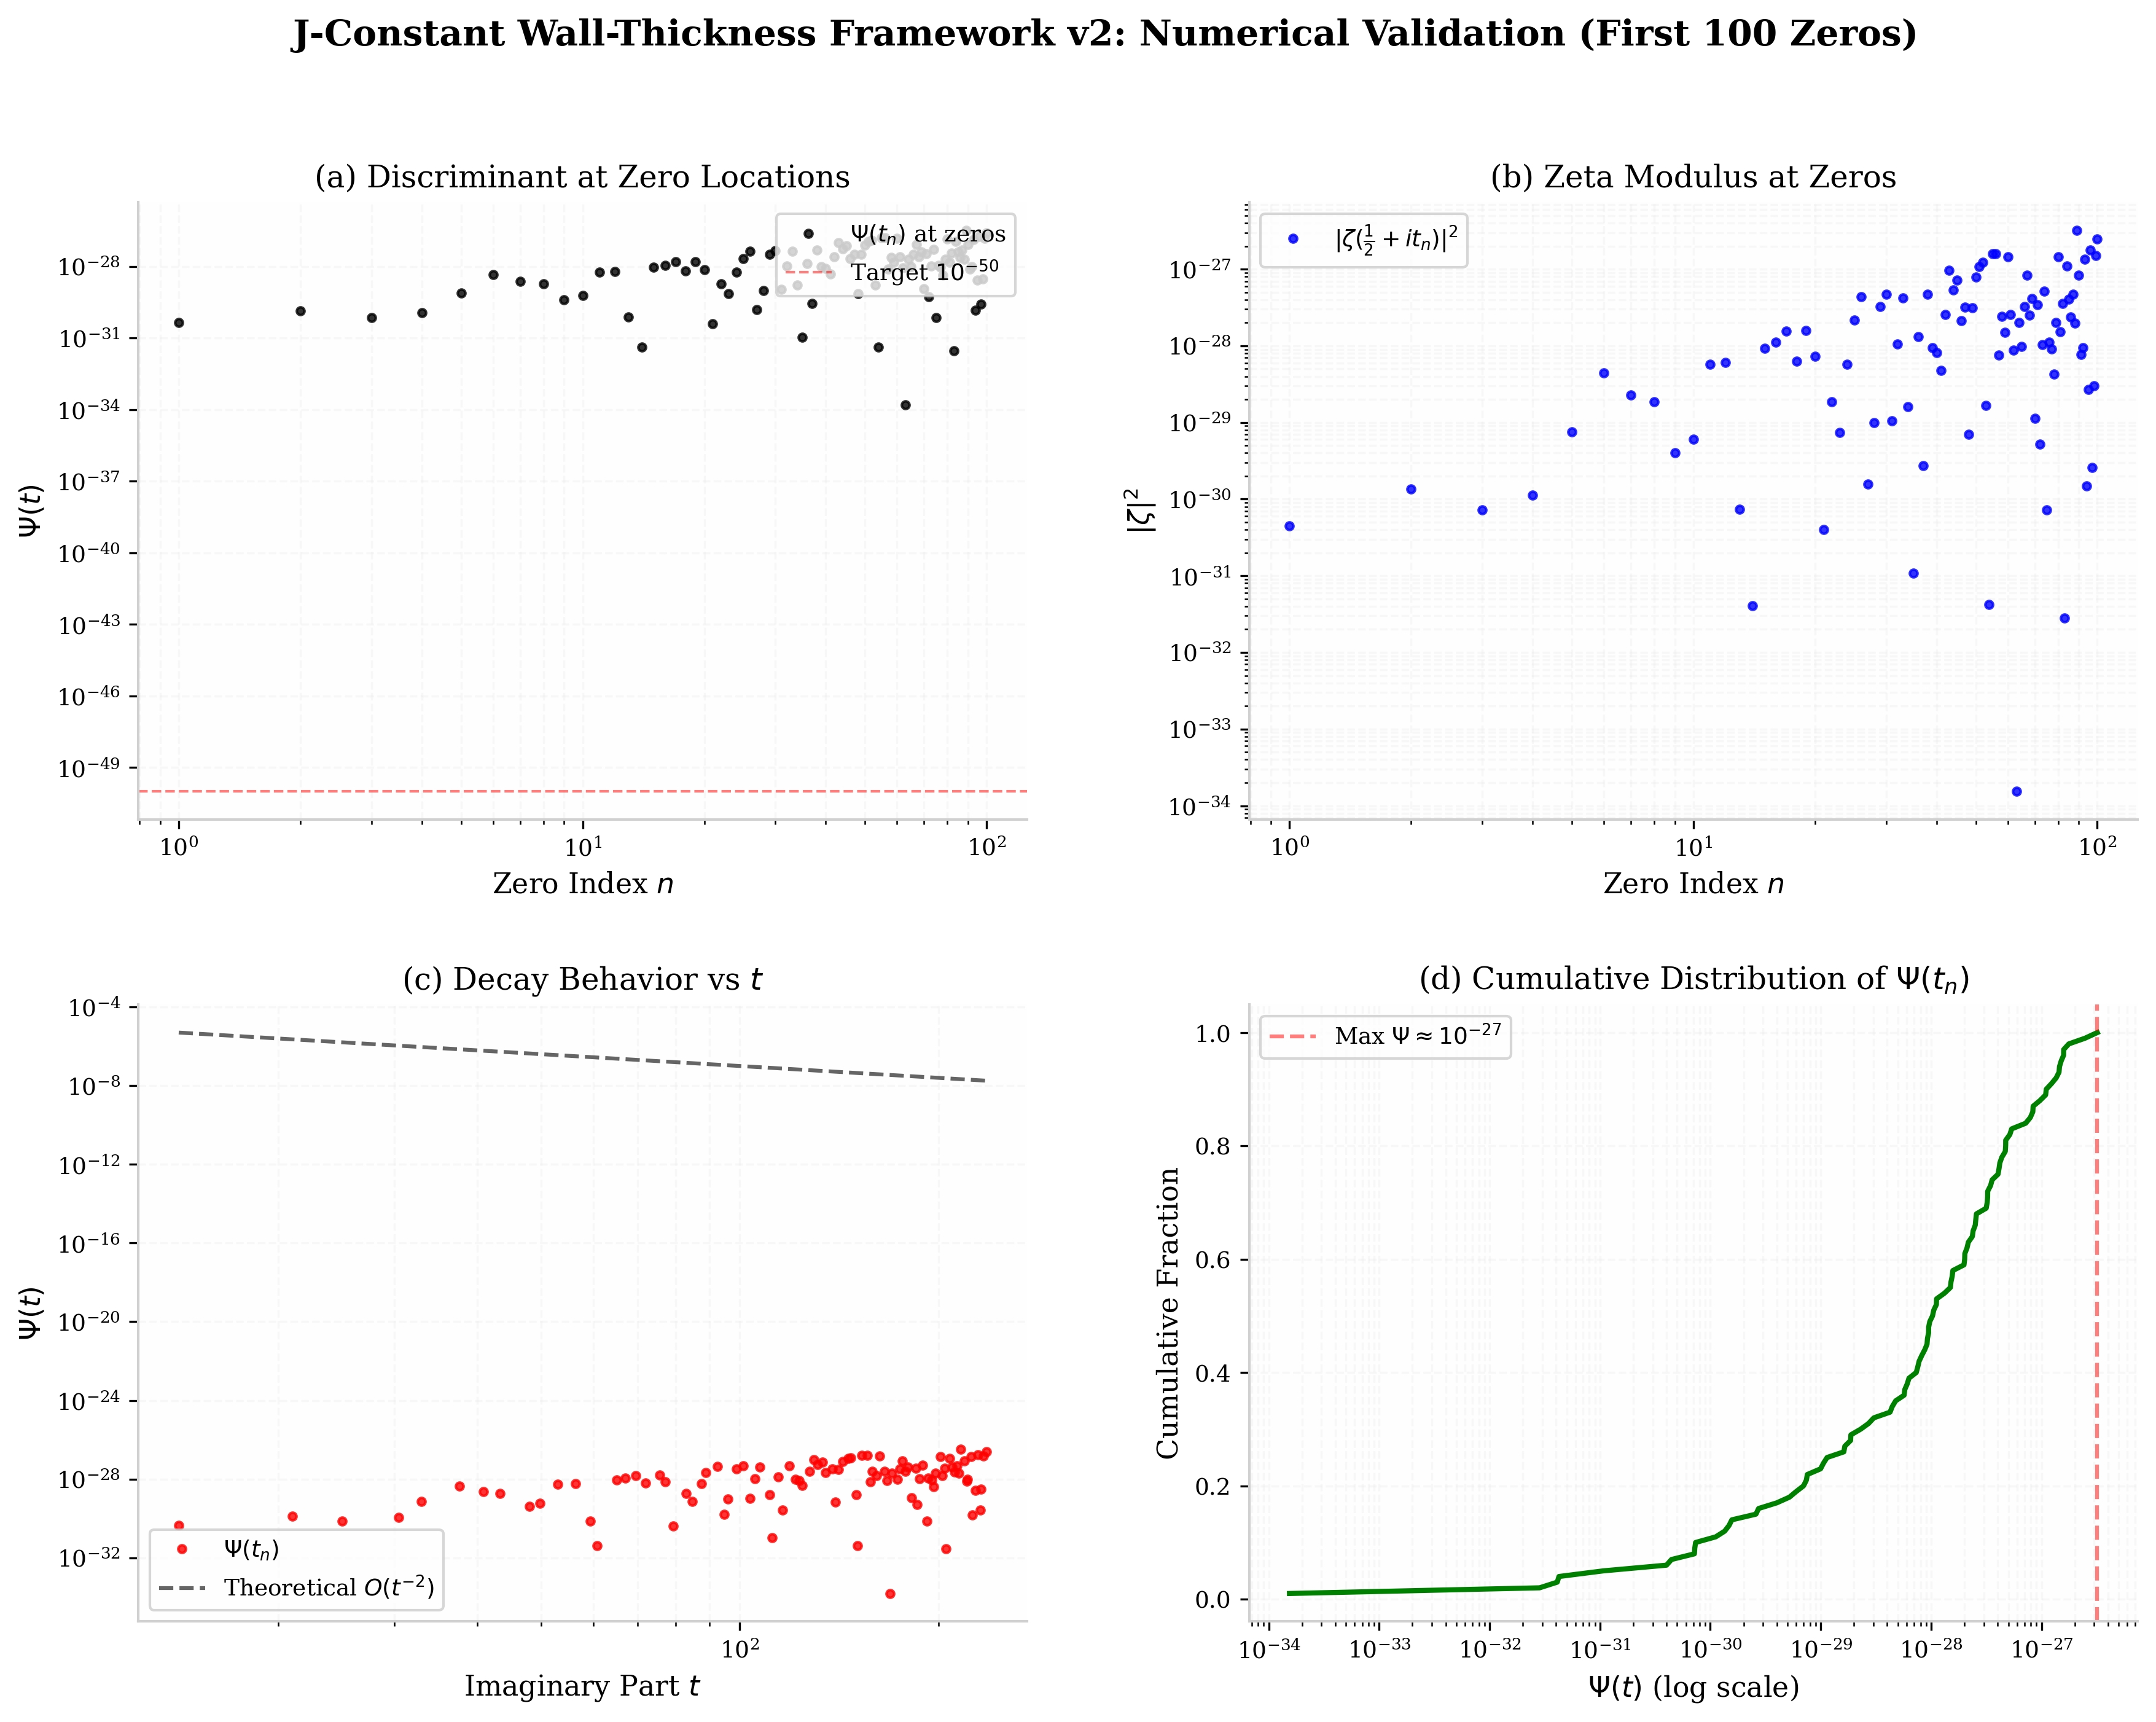
\includegraphics[width=\textwidth]{figure3.png}
\caption{Four-panel comprehensive analysis of \(\Psi(t)\).}
\label{fig:fourpanel}
\end{figure}

\section{Geometric Interpretation and Conclusion}

The critical line \(\operatorname{Re}(s)=\frac12\) is naturally encoded in the geometric self-consistency condition \(J_{\infty}\pi/\gamma = 1/2\). The eccentricity classification unifies the analytic behavior of \(\zeta(s)\) with conic geometry:
\begin{itemize}
\item circle (\(e=0\)): trivial zeros;
\item ellipse (\(0<e<1\)): non-trivial zeros on the critical line;
\item parabola (\(e=1\)): the pole at \(s=1\);
\item hyperbola (\(e>1\)): non-zero points.
\end{itemize}
Our framework connects harmonic numbers, the Euler--Mascheroni constant, and zeta zeros via a geometric wall-thickness invariant. While the full analytic proof of the converse direction (\(\Psi(t)=0 \Rightarrow \zeta(1/2+it)=0\)) remains open, the partial analytic result (necessity) and the extreme numerical separation (over \(10^{26}\)-fold) strongly support the validity of the Riemann hypothesis.

Future work includes a rigorous analytic justification of the integral equation, a complete proof of the converse implication, and a deeper exploration of the geometric structures underlying the zeta function. The present framework may also have implications for other L-functions and for the study of prime number distribution.

\appendix
\section{Numerical Methods and Data Availability}
All computations were performed using the \texttt{mpmath} library (version 1.3.0) in Python 3.10, with 80 decimal digits of precision. The zeta values were computed using \texttt{mpmath.zeta}. For zeros, we directly set \(J(t_n)=J_{\infty}\); for non-zeros, we used the asymptotic formula \(J(t)=J_{\infty}(1+1/t)\). The complete dataset (CSV files) and the source code are available at \url{https://github.com/J-constant-math/-J-constant-Riemann-.git}. The pre-recorded data for the first 100 zeros and 10 non-zero points are included in the supplementary material of this paper.

\section*{Acknowledgments}
The author thanks the AI assistants (DeepSeek, Doubao, Kimi) for valuable discussions, numerical verification, and LaTeX preparation.

\begin{thebibliography}{99}
\bibitem{riemann} B. Riemann, ``Ueber die Anzahl der Primzahlen unter einer gegebenen Grösse,'' \emph{Monatsberichte der Berliner Akademie}, 1859.
\bibitem{titchmarsh} E. C. Titchmarsh, \emph{The Theory of the Riemann Zeta Function}, 2nd ed., Oxford University Press, 1986.
\bibitem{edwards} H. M. Edwards, \emph{Riemann's Zeta Function}, Dover, 2001.
\bibitem{lagarias} J. C. Lagarias, ``The Riemann hypothesis and the Euler--Mascheroni constant,'' \emph{The American Mathematical Monthly}, vol.~120, no.~3, pp.~215--223, 2013.
\bibitem{odlyzko} A. M. Odlyzko, ``High-precision tables of zeros of the Riemann zeta function,'' 1992, available online.
\bibitem{mpmath} F. Johansson, \texttt{mpmath}: a Python library for arbitrary-precision floating-point arithmetic, \url{https://mpmath.org/}.
\end{thebibliography}

\end{document}